\documentclass[12pt,pdftex,a4paper]{scrartcl}
\usepackage[english]{babel}
\usepackage[utf8]{inputenc}
\usepackage{amsmath}
\usepackage{amssymb}
\usepackage{amsthm}
\usepackage{mathtools}
\usepackage{listings}
\usepackage[onehalfspacing]{setspace}
\usepackage{xr}
\usepackage{float}
\usepackage{paralist}

\allowdisplaybreaks

% Figure as tikz
\usepackage{tikz}
\usepackage{pgfplots}
\pgfplotsset{compat = newest}
\newlength\figureheight
\newlength\figurewidth

% Figure Lable
\usepackage{subfigure}
\usepackage[small, bf]{caption}

%\usepackage{cite}
\usepackage{csquotes}
\usepackage{trfsigns}

% Für Einleitung
\usepackage{geometry}


% Own Commands
\newcommand{\ic}{\textit{i}}
\newcommand{\expo}{\mathrm{e}}
\newcommand{\dif}{\,\mathrm{d}}
\newcommand{\set}[1]{\mathbb{#1}}
\newcommand{\mcal}[1]{\mathcal{#1}}
\newcommand{\mat}[1]{\textbf{#1}}
\lstset{language=Python,basicstyle=\footnotesize}
\renewcommand{\arraystretch}{1.2}
\addtolength{\footskip}{15mm}
\DeclareMathOperator*{\argmin}{argmin}


\begin{document}
%\renewcommand{\labelenumi}{\textbf{\arabic{enumi}}}
%\renewcommand{\labelenumi}{\bfseries{\theenumi.}}
\renewcommand{\labelenumi}{\alph{enumi})}
%\renewcommand{\labelenumii}{(\arabic{enumii})}
%\renewcommand{\labelenumi}{(\theenumi)}
\newcommand{\scale}{2.36}

%\numberwithin{equation}%{section}
%\bibliographystyle{splncs03}
%\bibliographystyle{abbrv}
\renewcommand*{\figurename}{Fig.}
\renewcommand{\tablename}{Tab.}

\setcounter{MaxMatrixCols}{24}

\begin{titlepage}

\begin{center}


% Oberer Teil der Titelseite:
\textsc{\LARGE Universität Stuttgart}\\[1.5cm]

\textsc{\Large Optimal Control}\\[0.5cm]


% Title
\newcommand{\HRule}{\rule{\linewidth}{0.5mm}}
\HRule \\[0.4cm]
{ \huge \bfseries Solution of Homework Exercise 2}\\[0.4cm]

\HRule \\[1.5cm]

\textsc{\Large Winter Term 17/18}\\[2.5cm]

% Author and supervisor
\begin{minipage}{0.4\textwidth}
\begin{center} \large
\emph{Authors:}\\
Silvia \textsc{Gramling} [2867885]\\
Markus \textsc{Schmidgall} [2880655]
\end{center}
\end{minipage}
\hfill
%\begin{minipage}{0.4\textwidth}
%\begin{flushright} \large
%\emph{Supervisor:} \\
%Jun.-Prof. Dr.~Andrea \textsc{Barth} \\
%Dr.~Ilja \textsc{Kröker}
%\end{flushright}
%\end{minipage}

\vfill

% Unterer Teil der Seite
{\large \today}

\end{center}

\end{titlepage}

%\tableofcontents
\setcounter{page}{1}
%\pagestyle{headings}
%\newpage

\newpage
\section*{Problem 1}
\begin{enumerate}

	\item The exercise yields a discrete-time infinte-horizon optimal control problem
	\begin{equation*}
		\begin{split}
			\min_{u_k} \,& \sum_{k=0}^\infty 0.9^k\,f_0(x_k,u_k) \\
			\text{s.t.} & \quad x_{k+1} = f(x_k,u_k) \\
			& \quad x_k \in \mathcal{X} \\
			& \quad u_k \in \mathcal{U}
		\end{split}
	\end{equation*}
	The function $f$ is the transition function which donates the state $x_{k+1}$ given $x_k$ and $u_k$. It can be read from the graph:
	
	\begin{center}
	\begin{tabular}{ l c r }
    $f(\xi_1, u_0) = \xi_2$, & $f(\xi_1, u_1) = \xi_2$, & $f(\xi_1, u_2) = \xi_3$, \\
	$f(\xi_2, u_0) = \xi_7$, & $f(\xi_2, u_1) = \xi_5$, & $f(\xi_2, u_2) = \xi_4$, \\
	$f(\xi_3, u_0) = \xi_4$, & $f(\xi_3, u_1) = \xi_6$, & $f(\xi_3, u_2) = \xi_5$, \\
	$f(\xi_4, u_0) = \xi_7$, & $f(\xi_4, u_1) = \xi_8$, & $f(\xi_4, u_2) = \xi_6$, \\
	$f(\xi_5, u_0) = \xi_4$, & $f(\xi_5, u_1) = \xi_4$, & $f(\xi_5, u_2) = \xi_6$, \\
	$f(\xi_6, u_0) = \xi_1$, & $f(\xi_6, u_1) = \xi_7$, & $f(\xi_6, u_2) = \xi_8$, \\
	$f(\xi_7, u_0) = \xi_8$, & $f(\xi_7, u_1) = \xi_8$, & $f(\xi_7, u_2) = \xi_8$, \\
	$f(\xi_8, u_0) = \xi_8$, & $f(\xi_8, u_1) = \xi_8$, & $f(\xi_8, u_2) = \xi_8$. \\
    \end{tabular}
	\end{center}
	
	The value function iteration
	\begin{equation*}
		V^{new}(\xi_k) = (TV^{old})(\xi_k), \quad \xi_k \in \mathcal{X}
	\end{equation*}
	is defined by the DP operator
	\begin{equation*}
		(TV)(\cdot ) = \min_{u\in\mathcal{U}}\{ f_0(\cdot , u) + 0.9\,V(f(\cdot , u))\}.
	\end{equation*}
	
	\item Trusting in the MATLAB program, the value function reads
	\begin{equation*}
		V^\star =
		\begin{bmatrix}
			4.16 & 4.9 & 2.4 & 1 & 3.9 & 2.35 & 1.5 & 0 
		\end{bmatrix}
	\end{equation*}
	where every entry represents the optimal cost when starting at the corresponding state.	
	The optimal control feedback is given by
	\begin{center}
	\begin{tabular}{ l l l }
    $v_k(\xi_1) = 2$, & $v_k(\xi_2) = 2$, & $v_k(\xi_3) = 0$, \\
	$v_k(\xi_4) = 1$, & $v_k(\xi_5) = 0$, & $v_k(\xi_6) = 1$, \\
	$v_k(\xi_7) = 0 \; (\text{or } 1 \text{ or } 2)$, & $v_k(\xi_8) = 0 \; (\text{or } 1 \text{ or } 2)$. & \\
    \end{tabular}
	\end{center}
	This leads to the optimal path (starting at $\xi_1$)
	\begin{equation*}
		\begin{bmatrix}
			\xi_1 & \xi_3 & \xi_4 & \xi_8 & \xi_8 & \cdots
		\end{bmatrix}
	\end{equation*}
	with the optimal input sequence
	\begin{equation*}
		\begin{bmatrix}
			u_2 & u_0 & u_1 & u_0 & u_0 & \cdots
		\end{bmatrix}.
	\end{equation*}	
	
	\item First of all, we show that $V^k \rightarrow V^\star$ and afterwards $V^0(\xi_i) \le V^\star(\xi_i)$ will be proven.
	
	We receive the series $\{V^j\}_{j\in \set{N}_0}$ by defining 
	\begin{equation*}
		V^{j+1}(\xi_i) := TV^j(\xi_i).
	\end{equation*}
	The series can also be expressed in the explicit form
	\begin{equation*}
		V^j(\xi_i) := T^jV^0(\xi_i).
	\end{equation*}
	To show the first statement, we claim that $T$ is a contraction on $\set{R}^\mathcal{X}$ which is the function space of all functions mapping from $\mathcal{X}$ to $\set{R}$, meaning that
	\begin{equation*}
		||TV^1 - TV^2||_\infty \le \beta\,||V^1 - V^2||_\infty, \quad 0 < \beta < 1.
	\end{equation*}
	
	\newpage
	This holds true since
	\begin{align*}
		||TV^1 - TV^2||_\infty = & \;\max_{x\in\mathcal{X}}\left| \min_{u\in\mathcal{U}}\{ f_0(x,u) + \alpha\,V^1(f(x,u))\} \right. \\
		& \left. - \min_{u\in\mathcal{U}}\{ f_0(x,u) + \alpha\,V^2(f(x,u))\}\right| \\
		\le & \;\max_{x\in\mathcal{X}}\left\{ \max_{u\in\mathcal{U}} | \alpha\,V^1(f(x,u)) - \alpha\,V^2(f(x,u)) | \right\} \\
		= & \;\alpha \max_{x\in\mathcal{X}}\left\{ \max_{u\in\mathcal{U}} | \,V^1(f(x,u)) -\,V^2(f(x,u)) | \right\} \\
		\le & \,\alpha ||V^1 - V^2||_\infty
	\end{align*}
	Due to the fact that $\alpha = 0.9 < 1$, the requirements for a contraction are satisfied. Now, we use the Banach fixed-point theorem which yields that there is exactly one $V^\star \in \set{R}^\mathcal{X}$ s.t. $TV^\star = V^\star$ and every series $\{V^j\}_{j\in \set{N}_0}$ with $V^0 \in \set{R}^\mathcal{X}$ and $V^{j+1} = TV^j$ converges to $V^\star$ which was to be proven.\\
	For the second proof we use the given inequality
	\begin{equation*}
		V^0(\xi_i) \le TV^0(\xi_i) =: T^1(\xi_i) \quad \forall\xi_i\in\mathcal{X}.
	\end{equation*}
	By using the monotonicity property of $T$ we derive that
	\begin{equation*}
		V^0(\xi_i) \le V^1(\xi_i) \Rightarrow V^1(\xi_i) = TV^0(\xi_i) \le TV^1(\xi_i) = V^2(\xi_i).
	\end{equation*}
	Applying the same property again, we gain $V^2(\xi_i) \le V^3(\xi_i)$. We can now go on and make use of it consecutively. This results in a series of inequations
	\begin{equation*}
		V^0(\xi_i) \le V^1(\xi_i) \le V^2(\xi_i) \le \ldots \le V^\infty(\xi_i).
	\end{equation*}
	We already know that $V^\infty(\xi_i) = V^\star(\xi_i)$ and so we have $V^0(\xi_i) \le V^\star(\xi_i)$.\\
	\hspace*{133mm}$\square$
	
	\item We consider the feasible set $F = \{V : V(\xi_i) \le TV(\xi_i), \; 1\le i \le n\}$ of the given optimization problem. Furthermore, we assume that $\tilde{V}\in F$ with $\tilde{V} \neq V^\star$ (obviously $V^\star \in F$). From c) we conclude that $\tilde{V}(\xi_i) \le V^\star(\xi_i), \; i = 1,\ldots, n$ (with at least one $j\in\{1,2,\ldots ,n\}$ such that $\tilde{V}(\xi_j) < V^\star(\xi_j)$). This results in
	\begin{equation*}
		\sum_{i=1}^n \tilde{V}(\xi_i) < \sum_{i=1}^n V^\star(\xi_i)
	\end{equation*}
	and hence $\tilde{V}$ cannot be the optimal solution. Since this argument holds for all $\tilde{V} \in F/\{V^\star\}$ the only possible solution left is $V^\star$.\\
	\hspace*{133mm}$\square$
	
	\item The constraints in d) were
	\begin{equation*}
		V(\xi_i) \le TV(\xi_i) \quad i = 1,\ldots, n
	\end{equation*}
	with
	\begin{equation*}
		TV(\xi_i) = \min_{u\in\mathcal{U}(\xi_i)}\{ f_0(\xi_i,u) + \alpha\,V(f(\xi_i,u))\}.
	\end{equation*}
	This holds true if and only if
	\begin{equation*}
		V(\xi_i) \le  f_0(\xi_i,u) + \alpha\,V(f(\xi_i,u))\quad \forall u\in\mathcal{U}(\xi_i).
	\end{equation*}
	In other words, we can transform the $n$ constraints into $\sum_{i=1}^n |\,\mathcal{U}(\xi_i)|$ linear constraints.\\
	To obtain the form
	\begin{equation*}
		\begin{split}
			V^\star = \argmin_V \;& c^\top V\\
			\text{s.t.} \;& AV \le b
		\end{split}
	\end{equation*}
	we need to define the matrices $c$, $A$ and $b$. You'll find them on the solution sheet.
	
	\item In order to examine the \textsc{Matlab} program take a look into \emph{run1.m}, \emph{valFunIteration.m}, \emph{valFunItAsLinProg.m} and \emph{onehot.m}.\\
	The file \emph{valFunItAsLinProg} already computes and returns the the optimal control feedback. We use the fact that $V^\star$ is a fix point of $T$, i.e. there is at least one $u$ for every $i \in \{1,2,\ldots ,8\}$ such that
	\begin{equation*}
		V^\star(\xi_i) =  f_0(\xi_i,u) + \alpha\,V(f(\xi_i,u)).
	\end{equation*}
	In the LQ approach this translates into the following rule: For every $i \in \{1,2,\ldots ,8\}$ there has to be at least one $k \in \{i, i+8, i+16\}$, s.t.
	\begin{equation*}
		a_k V^\star(\xi_i) = b_k
	\end{equation*}
	where $a_k$ is the $k$-th row of $A$. Due to numerical inaccuracies, it is very likely that $a_k \bar{V}(\xi_i) \approx b_k$ (with $\bar{V}$ the numerical solution), so we look for $\argmin_{k \in \{i, i+8, i+16\}} |a_k \bar{V}(\xi_i) - b_k|$ from which we can derive the corresponding $u\in\{u_0,u_1,u_2\}$.
\end{enumerate}


\newpage
\section*{Problem 2}
\begin{enumerate}
    \item To compute the equilibrium of the unforced system we consider the equation
    \begin{equation*}
         \begin{bmatrix}
             x^1 \\ x^2
         \end{bmatrix}
         = A
         \begin{bmatrix}
             x^1 \\ x^2
         \end{bmatrix}
    \end{equation*}
    with $A$ as defined on the exercise sheet. The matrix equation is equivalent to the following system of equations:
    \begin{align*}
         x^1 + 3 \cdot x^2 &= x^1 \\
         -0.5 \cdot x^1 +x^2 &= x^2.
    \end{align*}
    We receive immediately the unique solution $x^1 = x^2 = 0$, so the equilibrium of the unforced system lies in the origin. The stability of the equilibrium will be investigated by computing the eigenvalues of $A$:
    \begin{equation*}         
         \det (\lambda I - A) = \det
         \begin{bmatrix}
            \lambda -1 & -3 \\
            0.5 & \lambda -1
         \end{bmatrix}
         = (\lambda -1)^2 +1.5 = \lambda^2 -2 \lambda +2.5 \overset{!}{=} 0.
    \end{equation*}
    The solution of the eigenvalue equation is $\lambda_{1/2} = 1 \pm \im \frac{\sqrt{6}}{2}$, so the unforced system is not stable.
    \item The given discrete-time system can be formulated in the MPC scheme as follows:
    \begin{equation*} 
    \begin{array}{rcl} 
    u_{MPC} (\cdot , x(t_j)) = &\argmin\limits_u& \sum\limits_{j=k}^{k+2} x_j^\top x_j + u_j^2 +x_{k+3}^\top P x_{k+3} \\ 
    &\mathrm{s.t.}& x_{j+1} = A x_j + B u_j \\ 
    & & |u_j| \leq 1,\, x_j \in \mathbb{R}^2,\, x_{k+3} \in \mathcal{X}_f \\
    & & x_k = \bar{x}
    \end{array}      
    \end{equation*}
    with $P$, $A$, $B$ and $\mathcal{X}_f$ as defined on the exercise sheet.
    
    \item Now, we show that the controller $u_j = K x_j$ is feasible.
   \begin{compactenum}[1.]
   \item The minimal eigenvalue of $P$ is used as a lower limit in the following equation to show the feasibility of the controller:
      \begin{equation*}         
         \lambda_{min}(P) |x|^2 \leq x^\top P x.
      \end{equation*}
   For all $x \in \mathcal{X}_f$ the relation
      \begin{equation*}         
         x^\top P x \leq c = \frac{\lambda_{min}(P)}{|K|^2}
      \end{equation*}
   holds by definition. After dividing by $\lambda_{min}(P)$ we obtain the input constraint
      \begin{equation*}         
         |u|^2 = |K|^2 |x|^2 \leq 1.
      \end{equation*}
      That means that $|u| \leq 1$, so the controller is feasible.
   \item By inserting the given definitions we gain
      \begin{align*}         
         \phi(x_{j+1})-\phi(x_j) &= x_{j+1}^\top P x_{j+1} - x_j^\top P x_j \\
         &= ((A-BK)x_j)^\top P (A-BK)x_j -  x_j^\top P x_j \\
         &= x_j^\top \underbrace{[(A-BK)^\top P (A-BK)-P]}_{\substack{L}} x_j \\
         & \leq \lambda_{max}(L) |x|^2.
      \end{align*}
   The eigenvalues of $L$ were computed via \textsc{Matlab}. Both of them are smaller than -7. Besides, we use that 
      \begin{equation*}         
         f_0(x_j,u_j) = |x_j|^2 + |K|^2 |x_j|^2 = (1 + |K|^2) |x_j|^2 = 3.05 |x_j|^2.
      \end{equation*}
   
   \newpage
   It follows that
      \begin{align*}         
         \phi(x_{j+1})-\phi(x_j) &\leq \lambda_{max}(L) |x|^2 \\
         & < -7 |x|^2 \\
         & < -3.05 |x^2| \\
         &= -f_0(x_j,u_j)
      \end{align*}
   which was to be proven.
   \item For showing that the terminal region $\mathcal{X}_f$ is invariant, we need to demonstrate that $x_{k+1} \in \mathcal{X}_f$ if $x_{k} \in \mathcal{X}_f$. From the previous task we know that
   \begin{equation*}
       \phi(x_{j+1})-\phi(x_j) = x_{j+1}^\top P x_{j+1} - x_j^\top P x_j \leq -f_0(x_j,u_j).
   \end{equation*}
   It follows from the definition of the terminal region ($x_j^T P x_j \leq c$) that 
   \begin{equation*}
       x_{j+1}^\top P x_{j+1} - c \leq -(|x_j|^2 + |u_j|^2).
   \end{equation*}
   This is equivalent to 
   \begin{equation*}
       x_{j+1}^\top P x_{j+1} \leq c - \underbrace{(|x_j|^2 + |u_j|^2)}_{\substack{\geq 0}} \leq c.
   \end{equation*}
   Consequently, $x_{k+1} \in \mathcal{X}$ and the terminal region $\mathcal{X}_f$ is invariant.\\
   \hspace*{133mm}$\square$
   \end{compactenum}

   \item The optimal control problem from b) can be written as a quadratically constrained quadratic program with the following variables
   \begin{align*}
		z &=
		\begin{bmatrix}
			x_k^\top & x_{k+1}^\top & x_{k+2}^\top & x_{k+3}^\top & u_k &  u_{k+1} & u_{k+2} 
		\end{bmatrix}^\top
		\in \set{R}^{11} \\
		H &=
		\begin{bmatrix}
			\mat{I}_{2} & 0 & & \cdots&  & & 0 \\
			0 & \mat{I}_{2} & & & & & \\
			&  & \mat{I}_{2} & \ddots & & & \\
			\vdots & & \ddots & P & & & \vdots \\
			& & & & 1 & & \\
			& & & &  & 1 & 0 \\
			0 & & & \cdots & & 0 & 1 \\
		\end{bmatrix}
		\in \set{R}^{11 \times 11} \\
		A_{eq} &= 
		\begin{bmatrix}
			\mat{I}_2 & 0 & 0 & 0 & 0 & 0 & 0 \\
			-A & \mat{I}_2 & 0 & 0 & -B & 0 & 0 \\
			0 & -A & \mat{I}_2 & 0 & 0 & -B & 0\\
			0 & 0 & -A & \mat{I}_2 & 0 & 0 & -B
		\end{bmatrix}
		\in \set{R}^{8 \times 11} \\	
		B_{eq} &= 
		\begin{bmatrix}
			\bar{x}^\top & 0 & \cdots & 0
		\end{bmatrix}^\top
		\in \set{R}^{11} \\
		A_{ineq} &=
		\begin{bmatrix}
			0 & & \cdots & 0 & 1 & 0 & 0 \\
			& & & & 0 & 1 & 0 \\
			\vdots & & & \vdots & 0 & 0 & 1 \\
			& & & & -1 & 0 & 0 \\
			& & & & 0 & -1 & 0 \\
			0 & & \cdots & 0 & 0 & 0 & -1 \\
		\end{bmatrix}
		\in \set{R}^{6 \times 11} \\
		B_{ineq} &=
		\begin{bmatrix}
			1 & \cdots & 1
		\end{bmatrix}^\top
		\in \set{R}^{6}	\\
		T &=
		\begin{bmatrix}
			0 & & & \cdots & & & 0 \\
			& 0 & & & & & \\
			& & 0 & & & & \\
			\vdots & & & P & & & \vdots \\
			& & & & 0 & & \\
			& & & & & 0 & \\
			0 & & & \cdots & & & 0 \\
		\end{bmatrix}
		\in \set{R}^{11 \times 11} \\
		d &= c \in \set{R}.
	\end{align*}
    The problem is convex, because 
    \begin{itemize}
    \item the matrizes $H$ and $T$ are positive definite ($P$ has only positive eigenvalues) and
    \item linear equations are always convex.
    \end{itemize}        
    
    \item Solving the optimization problem from d) with the \textsc{Matlab} file \emph{run2.m}, we obtain the resulting trajectory shown in Fig.~\ref{fig:pic_2e_X}. Obviously, the state $x$ converges to the equilibrium point in the origin. One can see in Fig.~\ref{fig:pic_2e_U} that the calculated input signal is large at first to move the state quickly to the equilibrium. The input constraints prevent higher magnitudes of the input than one. Both components of the state are moved to the origin and consequently, the input signal also converges to zero.
    \begin{figure}[H]
	\centering
	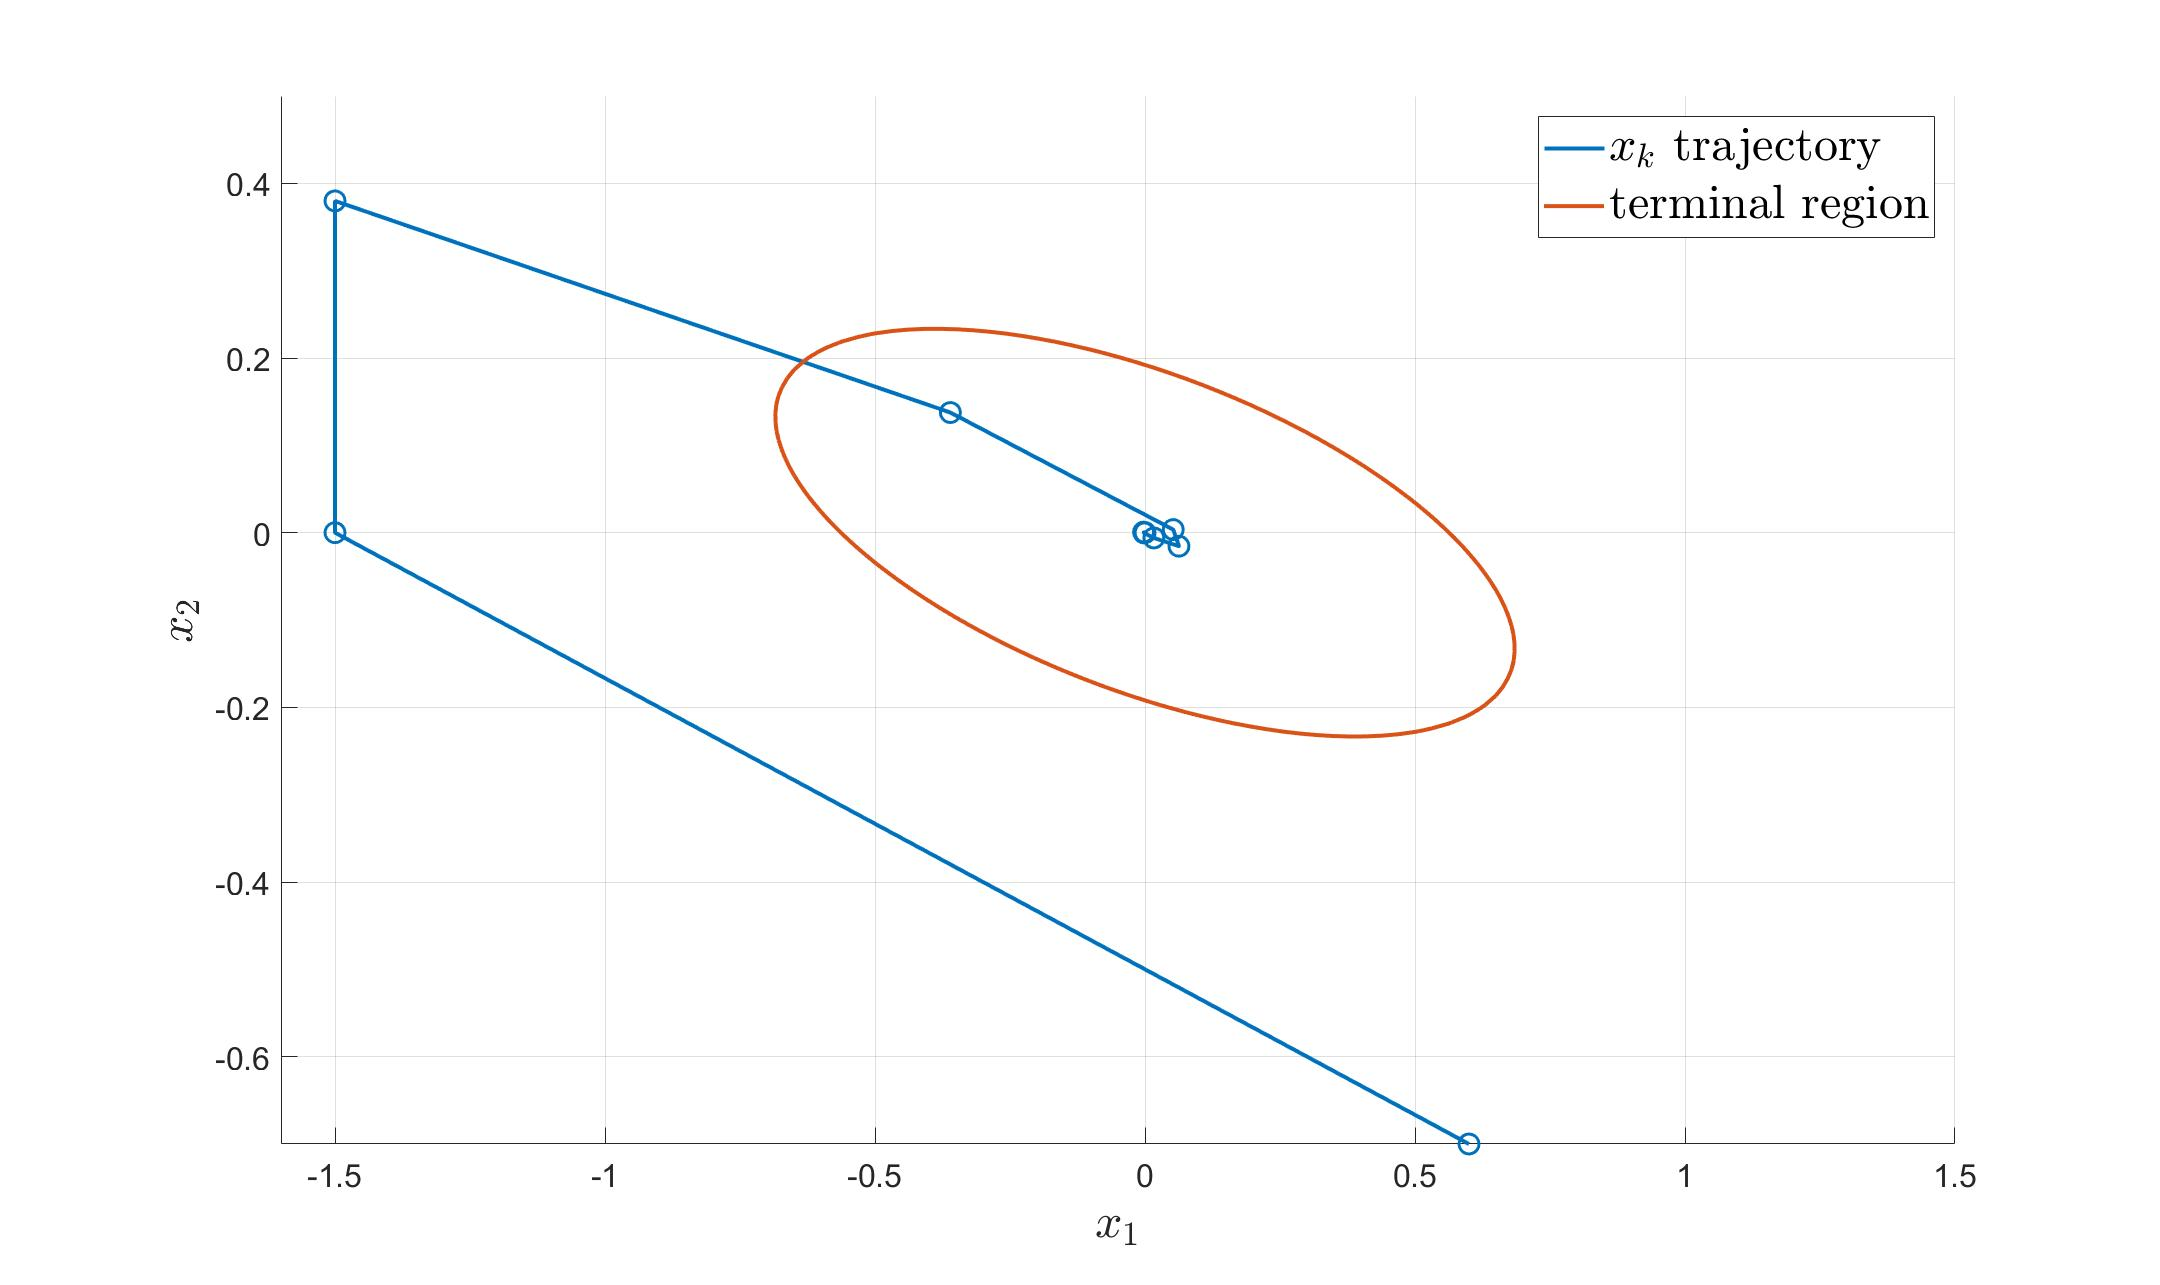
\includegraphics[scale=0.2]{pics/prop_2e_X.jpg}
	\caption{Trajectory of the optimal MPC solution}	
	\label{fig:pic_2e_X}
    \end{figure}

    \begin{figure}[H]
	\centering
	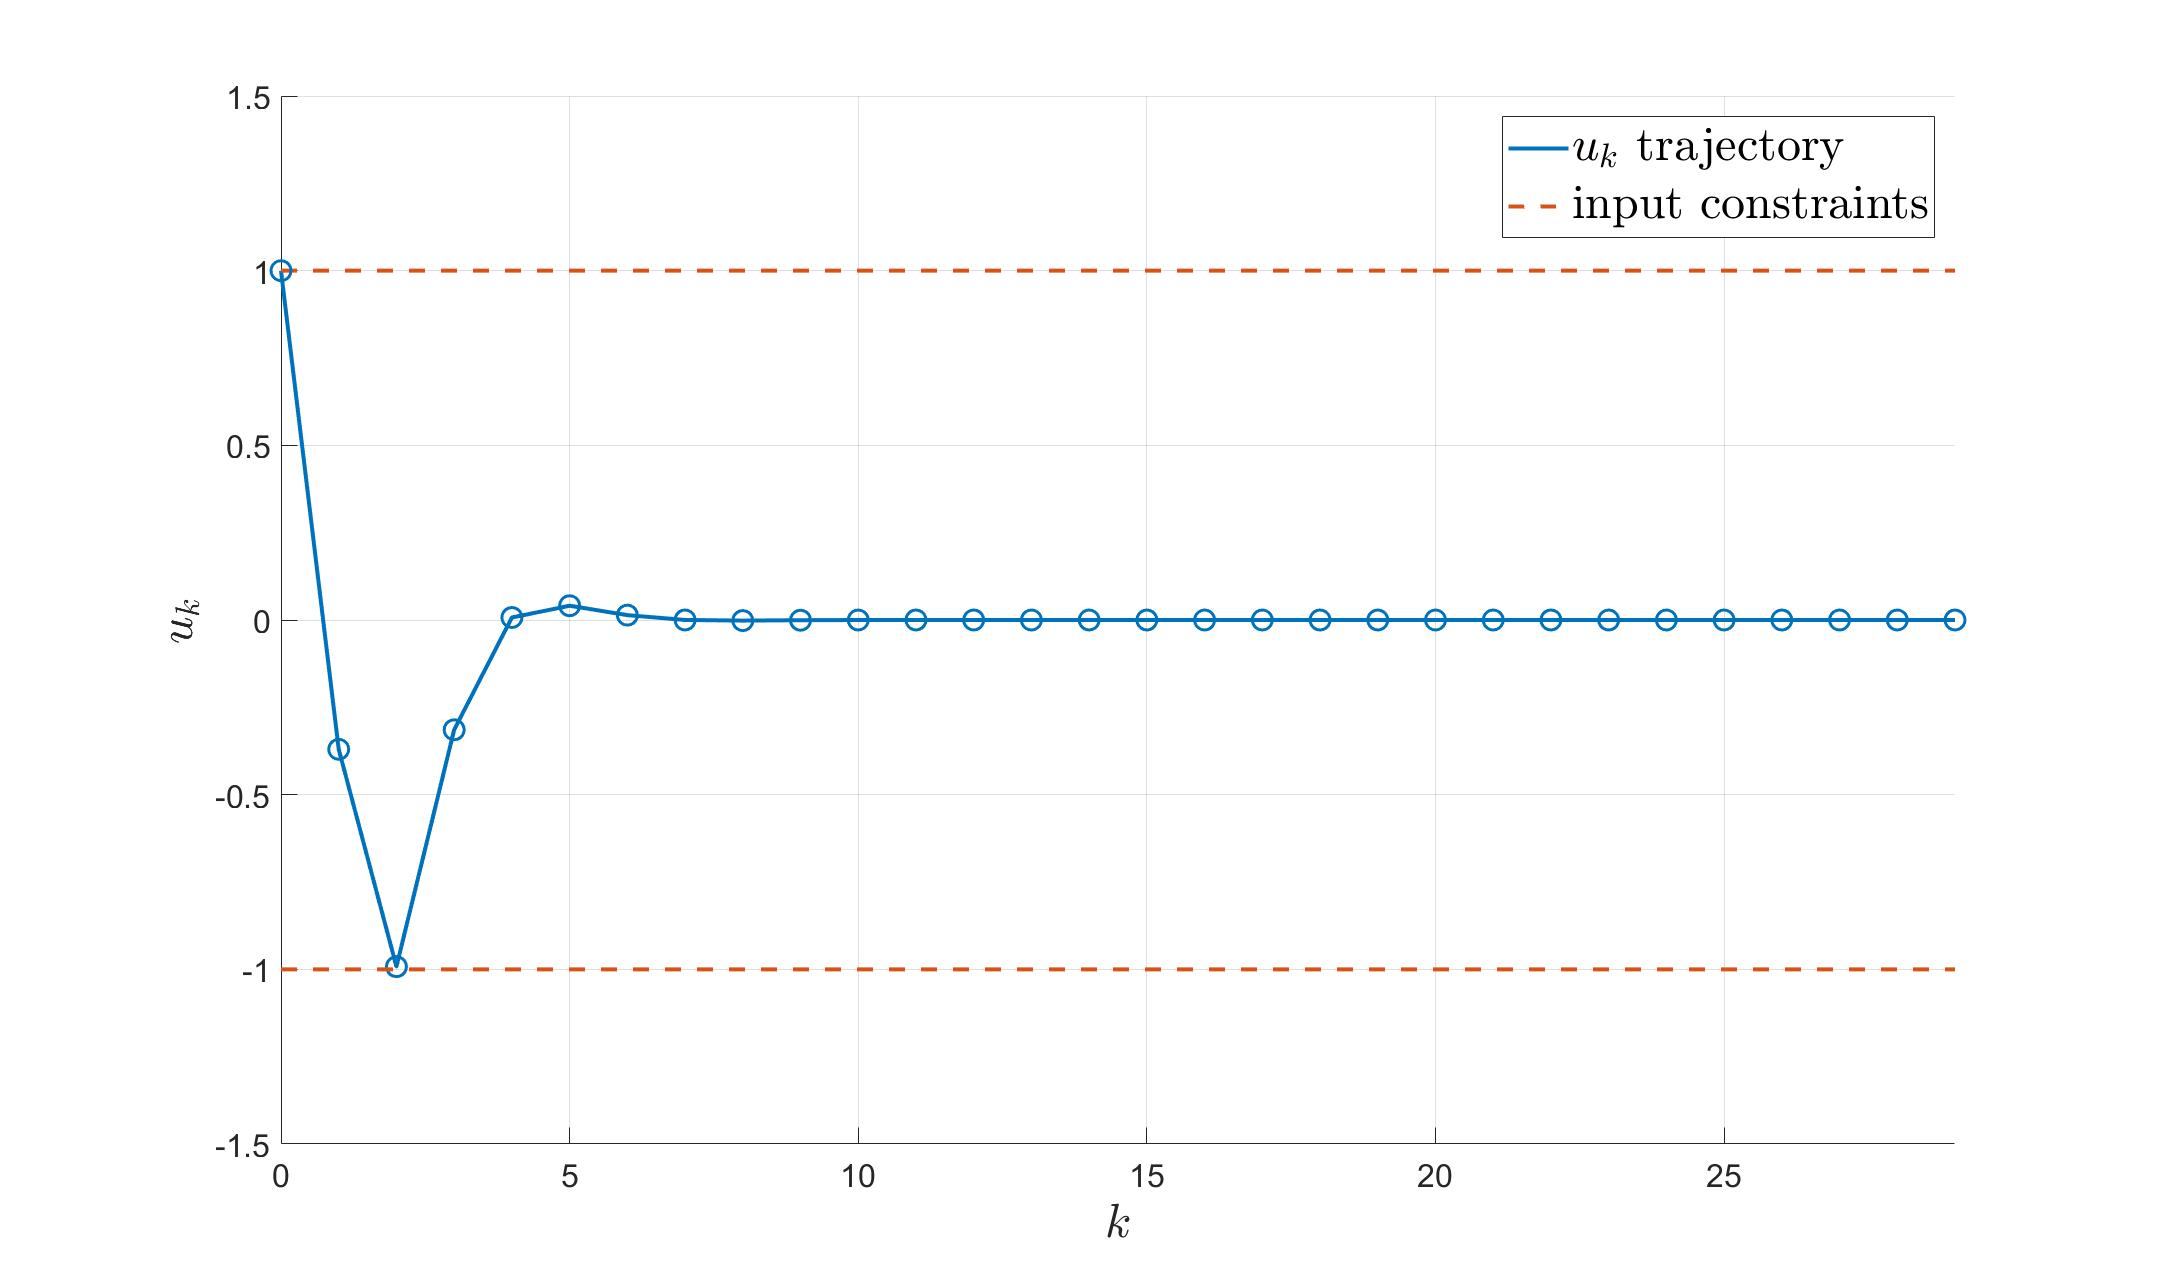
\includegraphics[scale=0.2]{pics/prop_2e_U.jpg}
	\caption{Optimal input signal of the MPC problem}	
	\label{fig:pic_2e_U}
    \end{figure}
    
    \item If we insert the other initial condition, we observe that that qualitative evolution of the state (Fig.~\ref{fig:pic_2f_X}) and the determined input (Fig.~\ref{fig:pic_2f_U}) is similar compared to the previous plots. That makes sense because both initial condition do not differ much from each other. In contrast to the previous task, it is not possible to satisfy all constraints: The new initial condition requests a higher input signal ($u_0 = 1.032$) so that the predicted $x_3$ is in the terminal region. The determined input signal $u_0$ is obviously higher than one, so the input constraint is violated.
    \begin{figure}[H]
	\centering
	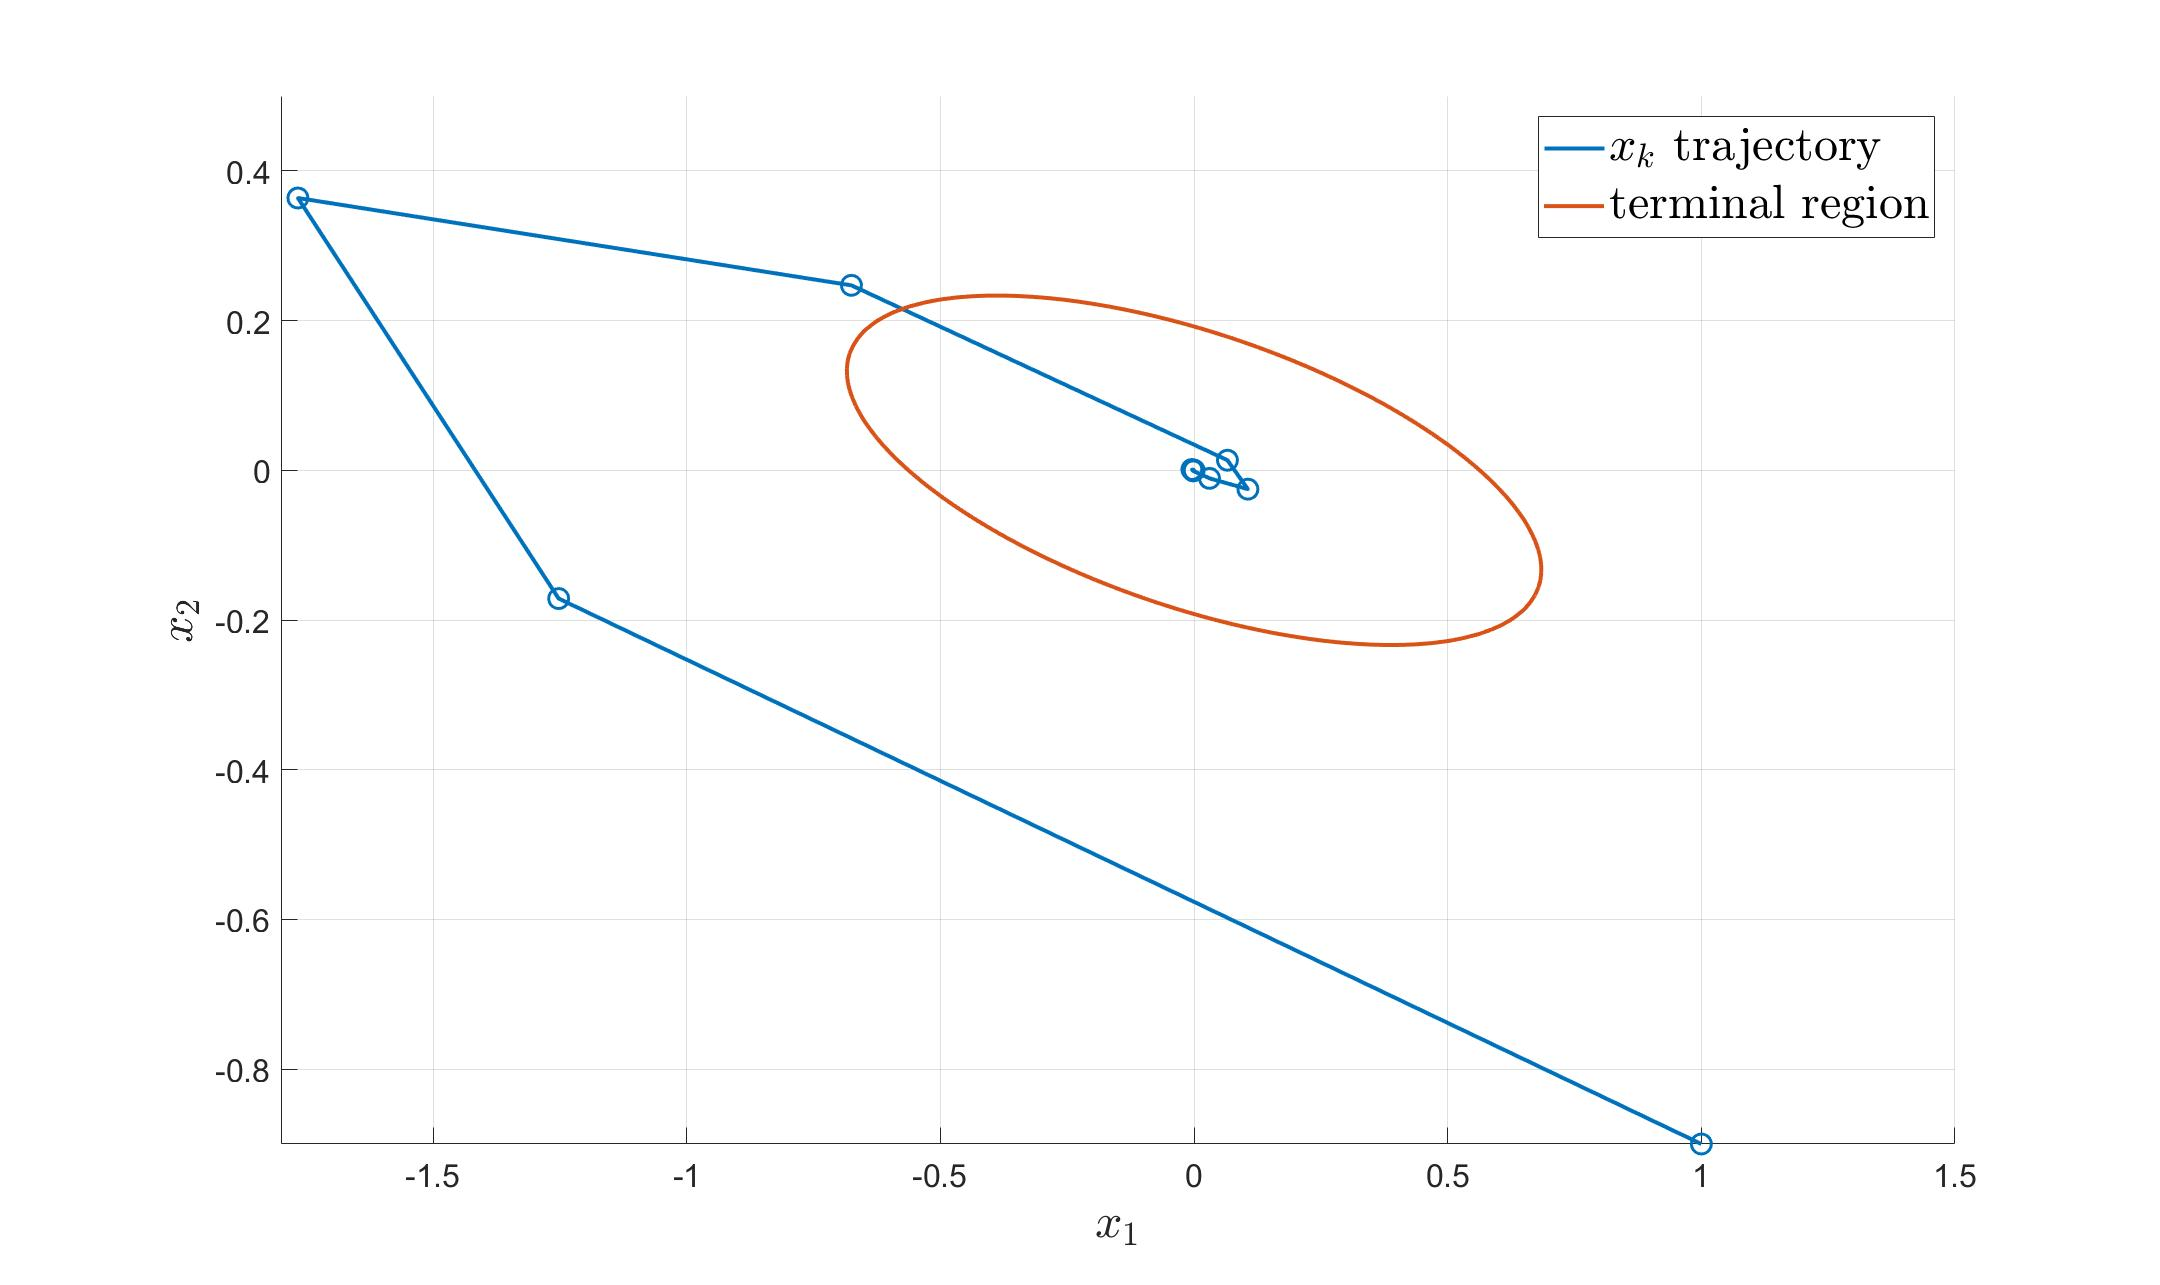
\includegraphics[scale=0.2]{pics/prop_2f_X.jpg}
	\caption{Trajectory of the optimal MPC solution for the new initial condition}	
	\label{fig:pic_2f_X}
    \end{figure}

    \begin{figure}[H]
	\centering
	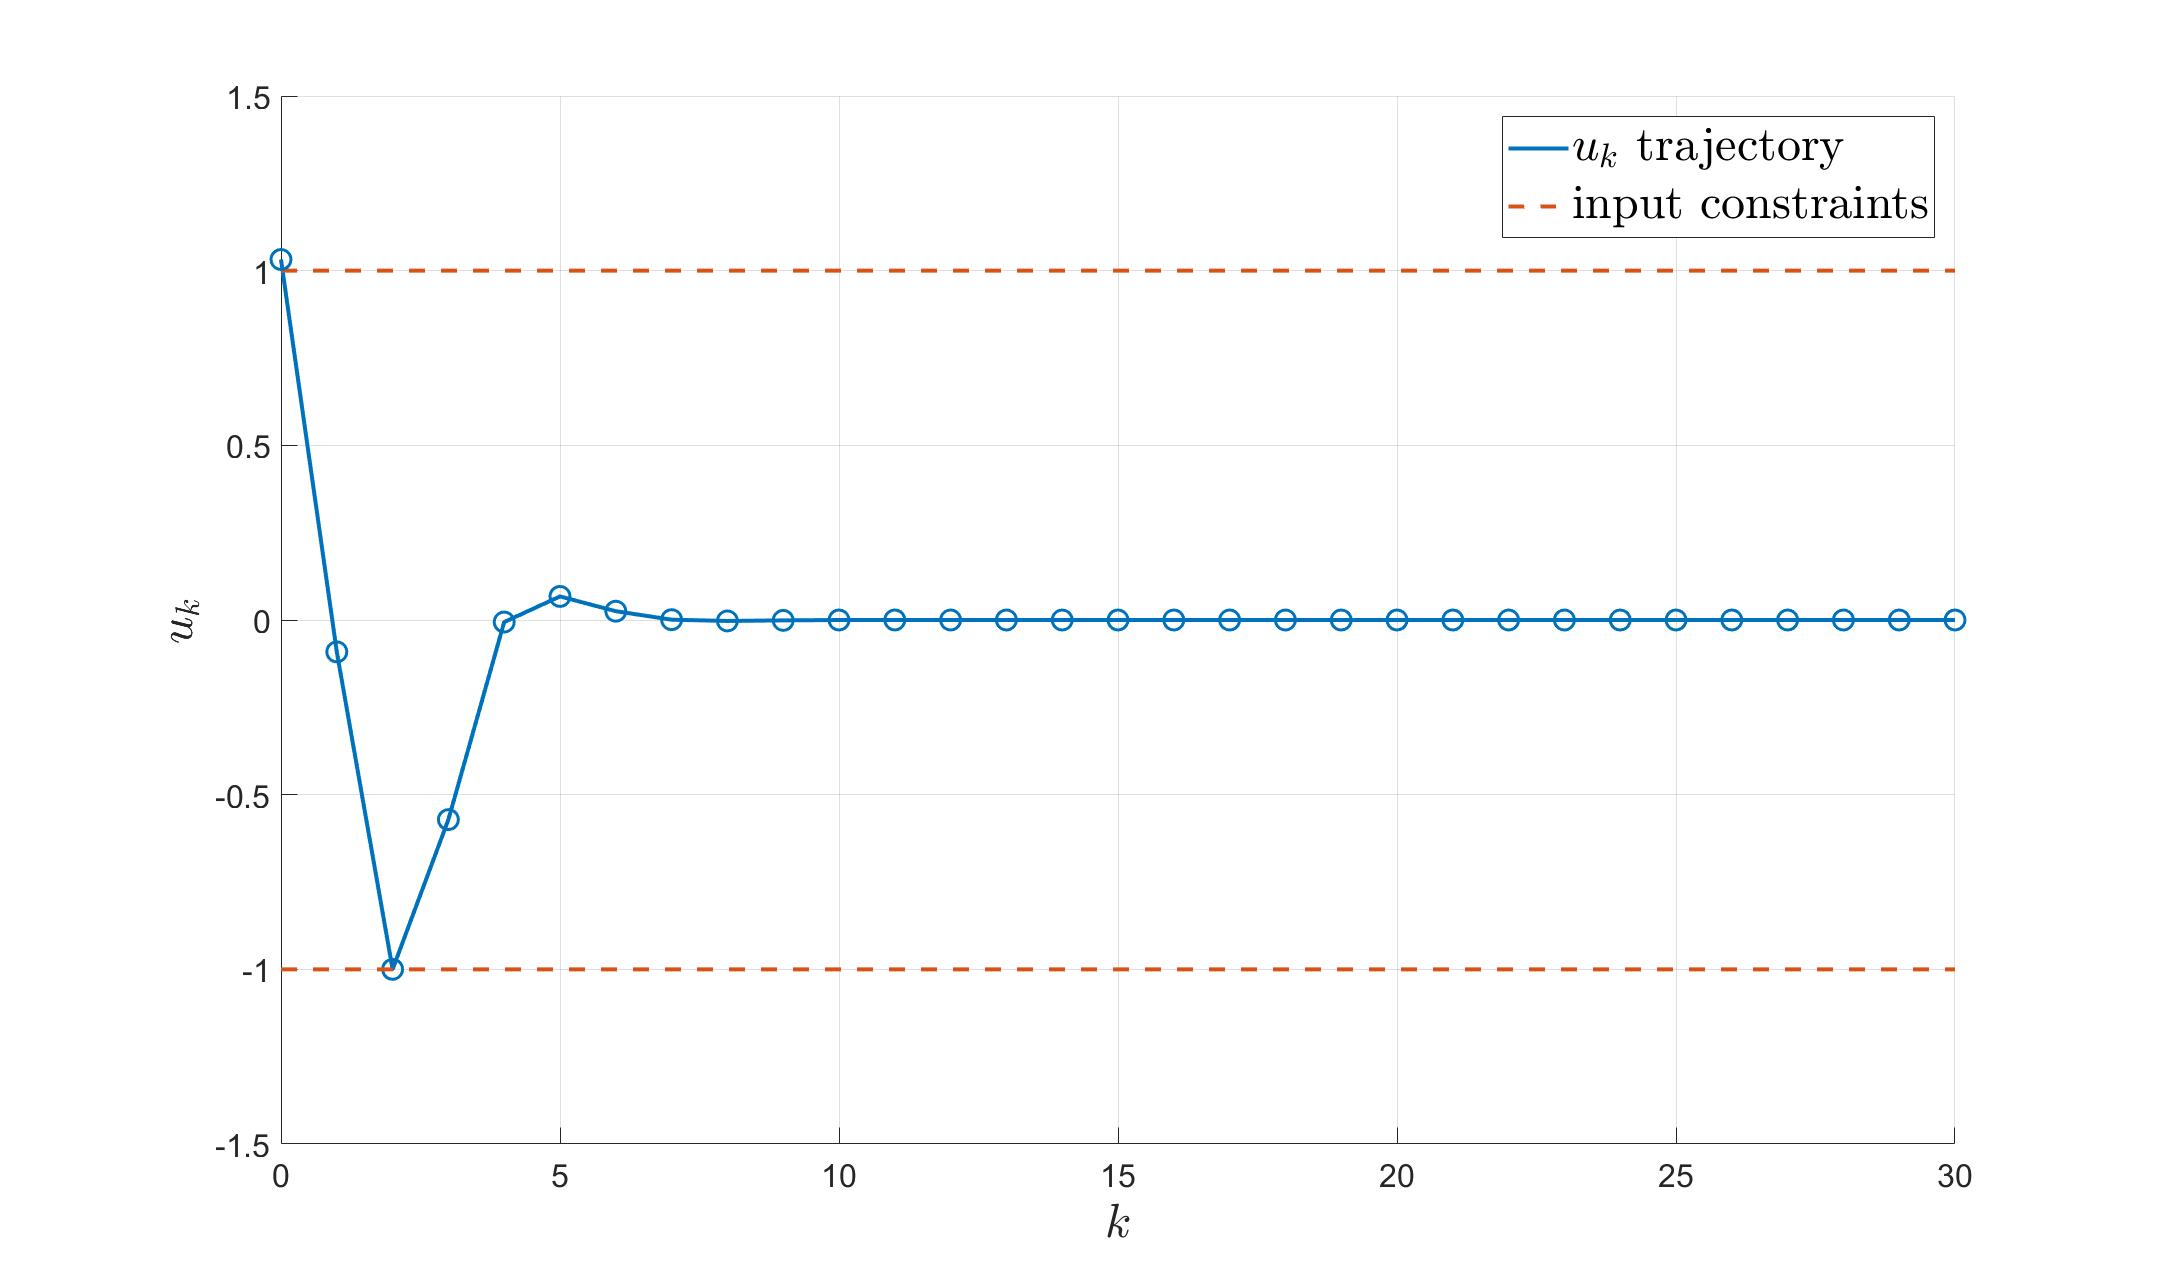
\includegraphics[scale=0.2]{pics/prop_2f_U.jpg}
	\caption{Optimal input signal of the MPC problem for the new initial condition}	
	\label{fig:pic_2f_U}
    \end{figure}
    
    \item Fig.~\ref{fig:pic_2g_X} shows the optimal state trajectory calculated via the LQ scheme. In contrast to the MPC algorithm, the \textsc{Matlab} solver for linear-quadratic problems does not include an input constraint. That is why the absolute value of the input signal is not restricted in contrast to the input in the previous tasks. In the LQ solution, we observe that the input is higher than one at first (Fig.~\ref{fig:pic_2g_U}), because that leads to a smaller value of the cost functional. Another difference is that the MPC scheme only minimizes the cost functional till the prediction horizon which is $N=3$ in our case. However, the prediction horizon does not have a huge impact on the trajectories and the qualitative evolution of the results stays the same.
    \begin{figure}[H]
	\centering
	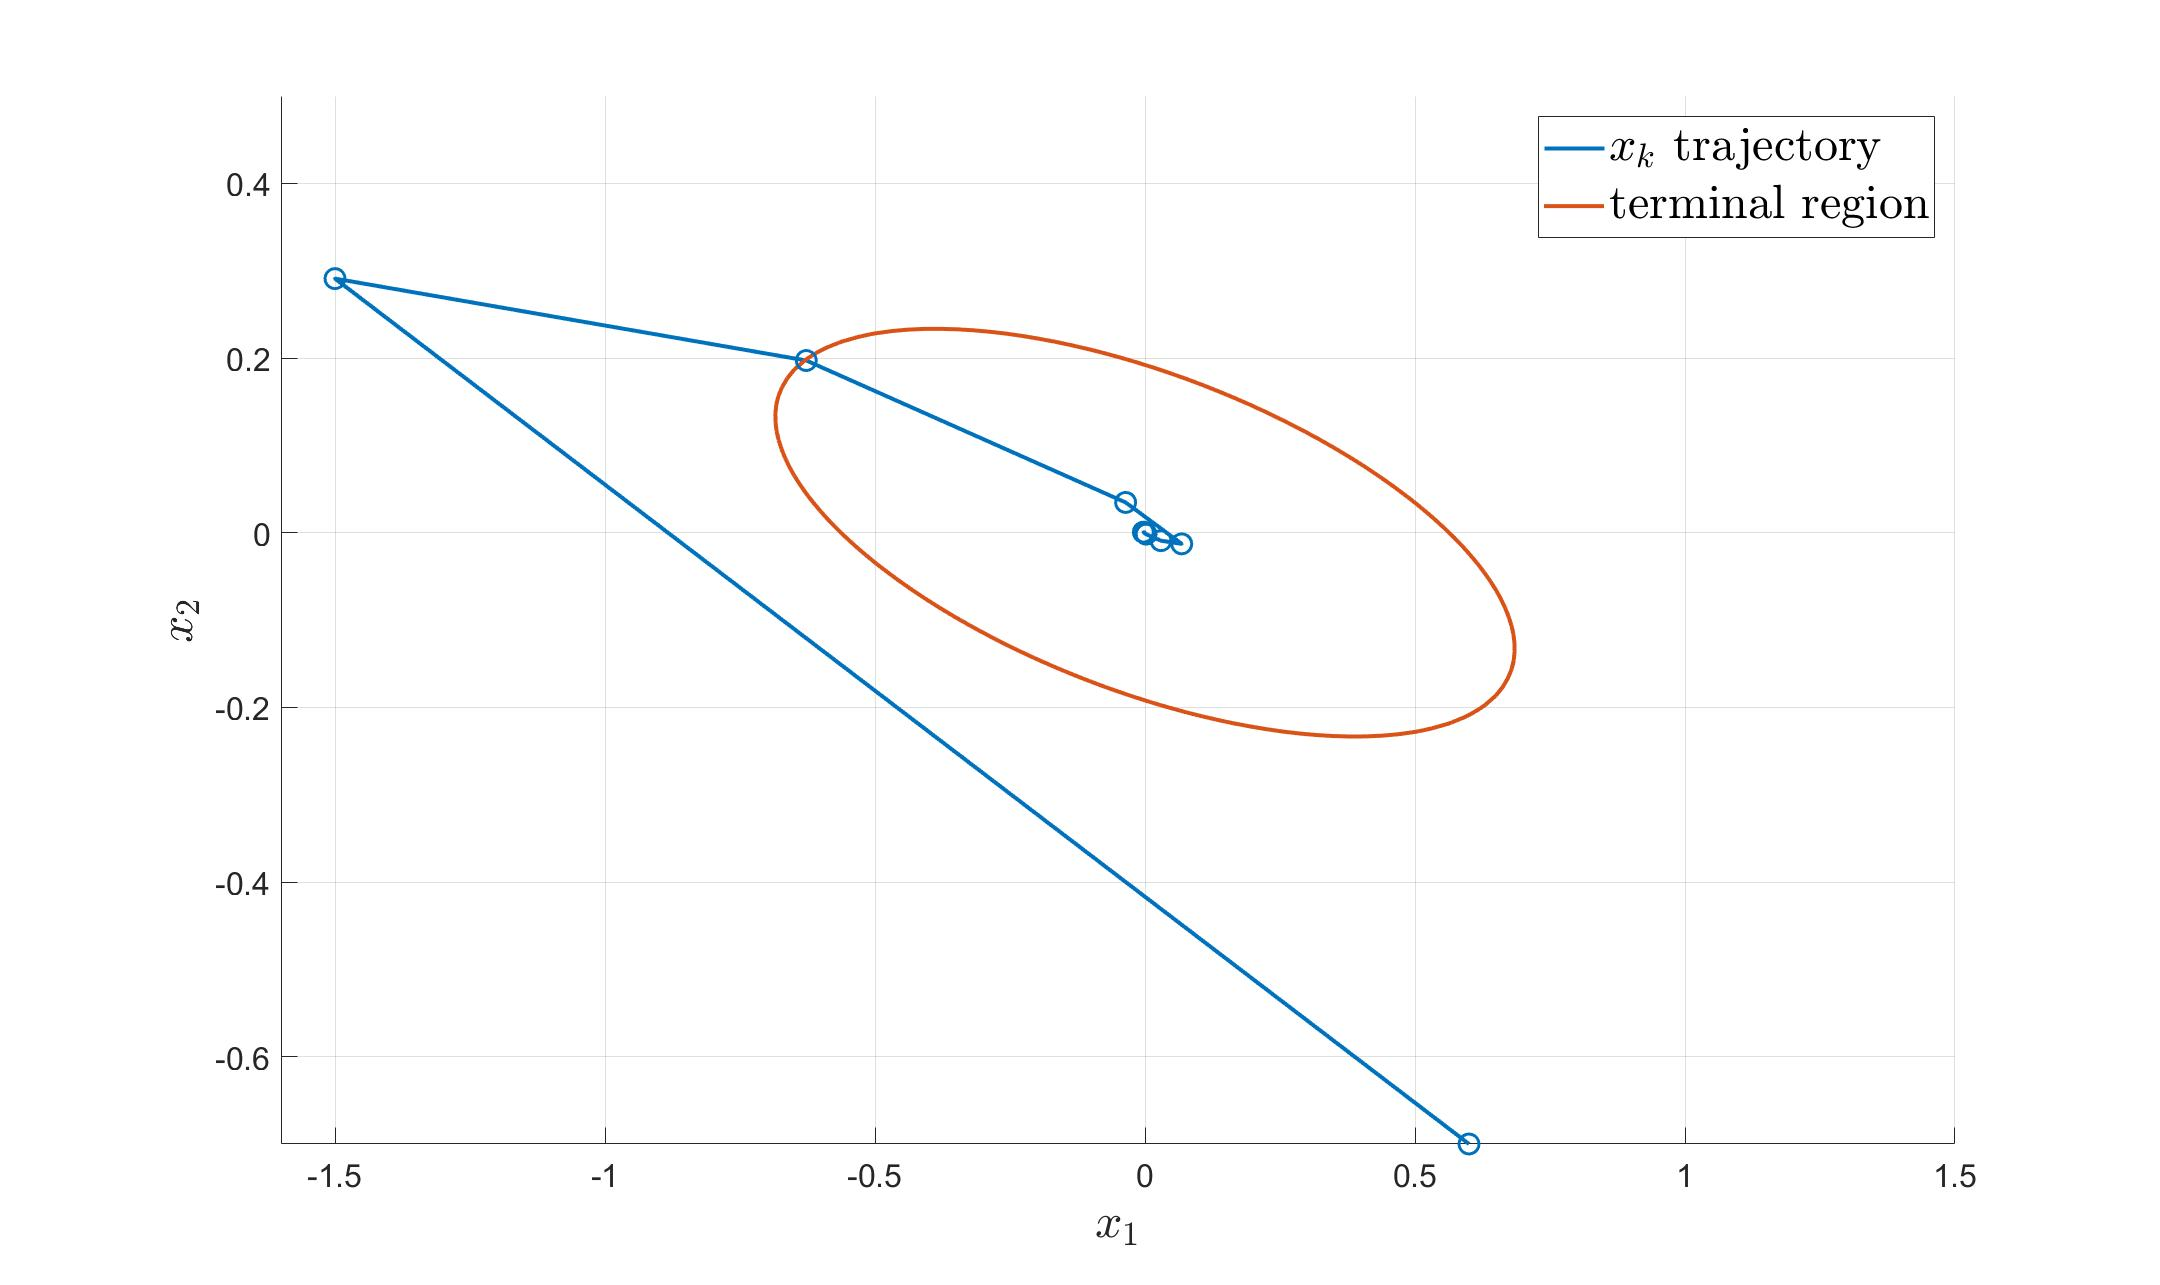
\includegraphics[scale=0.2]{pics/prop_2g_X.jpg}
	\caption{Trajectory of the optimal LQ solution}	
	\label{fig:pic_2g_X}
    \end{figure}

    \begin{figure}[H]
	\centering
	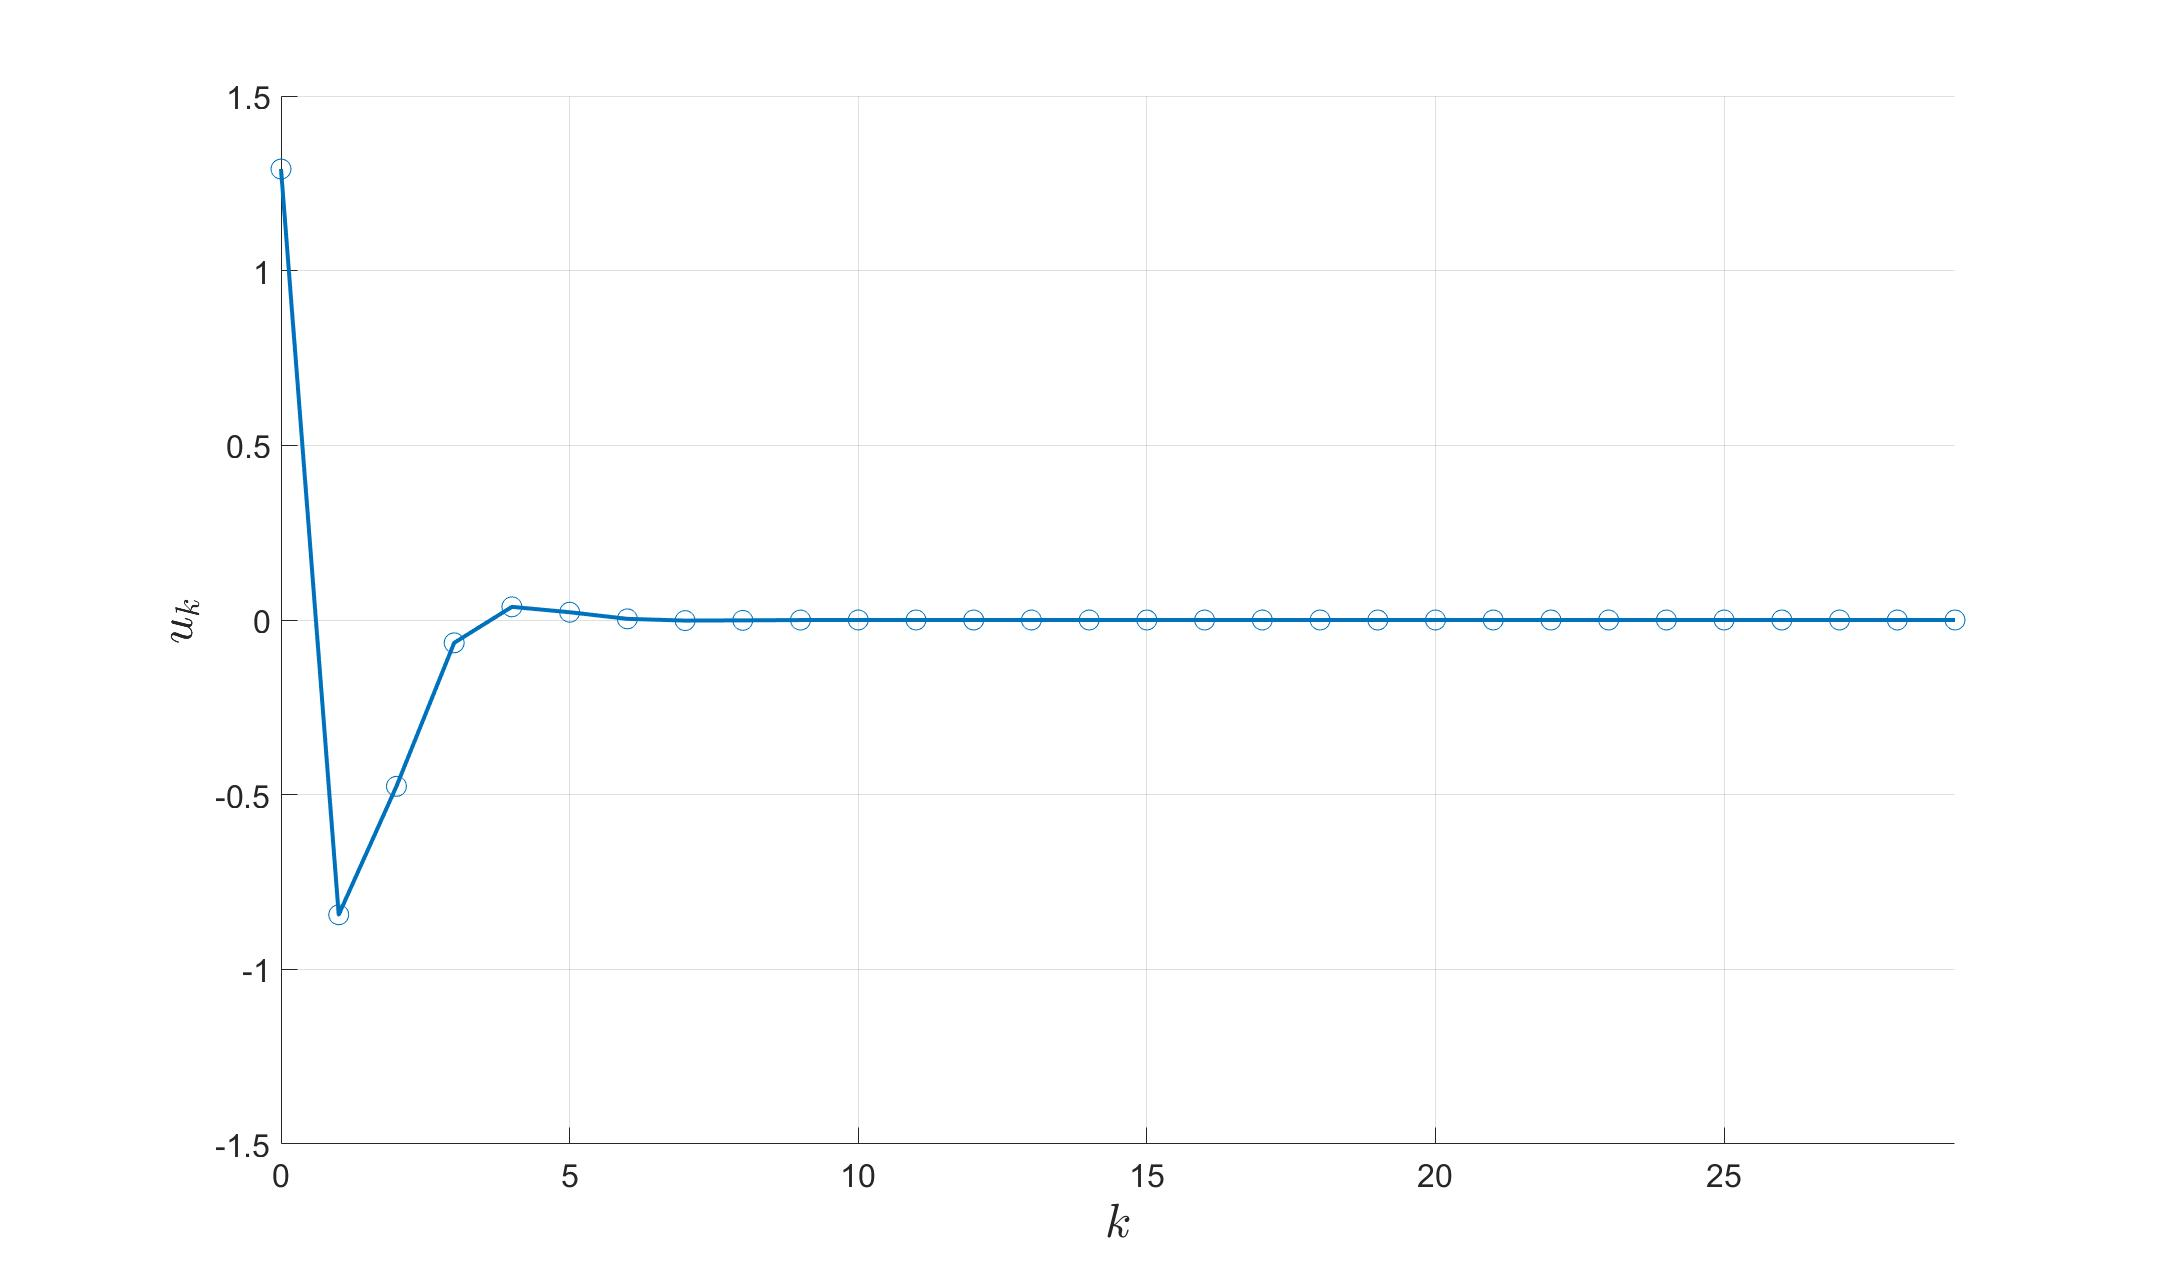
\includegraphics[scale=0.2]{pics/prop_2g_U.jpg}
	\caption{Optimal input signal of the LQ problem}	
	\label{fig:pic_2g_U}
    \end{figure}
    
\end{enumerate}

\end{document}